%!TEX root = ../main.tex

\chapter{Architettura del sistema}

Chiariamo come prima cosa la differenza tra un antenna per la televisione satellitare e un'antenna Starlink.
Le parabole TV utilizzano un riflettitore parabolico per focalizzare le onde elettromagnetiche che costituiscono i segnali televisivi inviati dai satelliti di trasmissione in orbita attorno alla terra e un'altitudine di 35000 km.
Le parabole TV ricevono solo segnali televisivi dallo spazio, non possono inviare dati.
La parabola Starlink, invece, invia e riceve dati Internet da un satellite Starlink in orbita a 550 km di distanza.
I collegamenti tra la parabola Starlink e il satellite devono essere concentrati in collegamenti potenti e stretti, continuamente orientati per massimizzare il puntamento utente-satellite \cite{branch_education_how_2022}.
Attualmente ci sono 6398 satelliti Starlink in orbita \cite{jonathan_mcdowell_starlink_nodate}.

\begin{figure}[htbp]
  \centering
  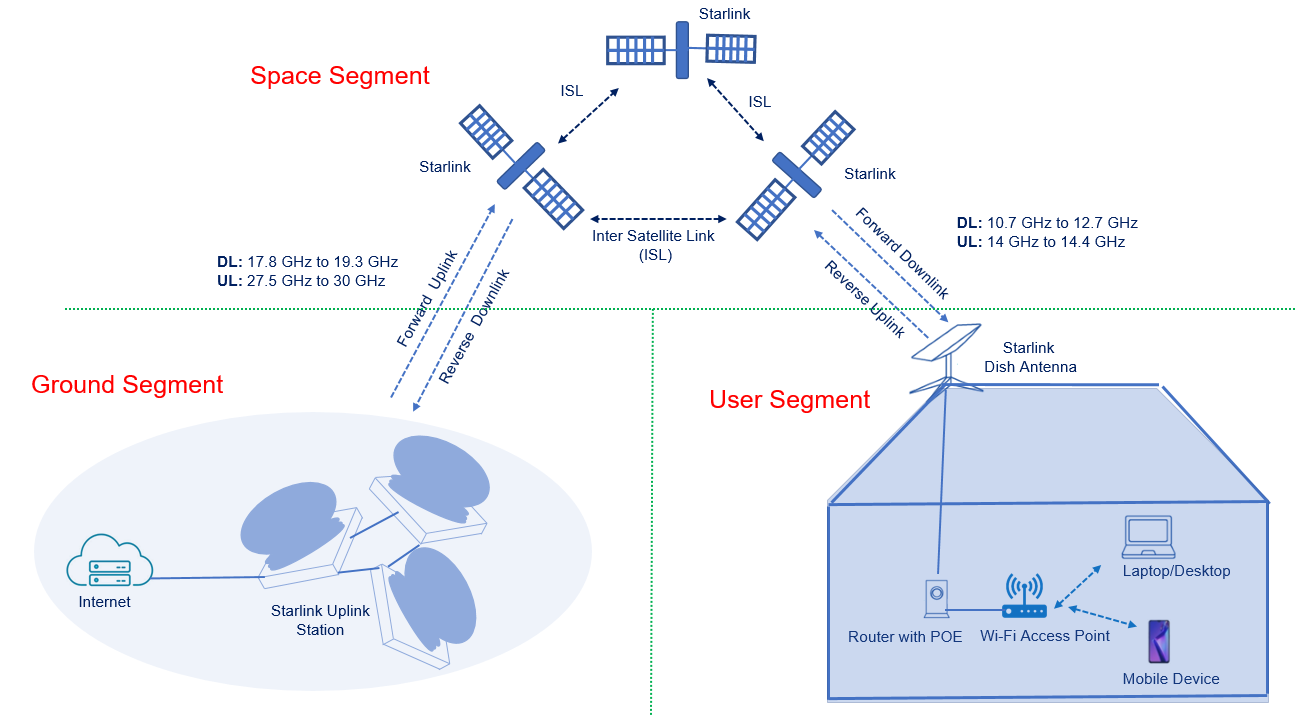
\includegraphics[width=0.9\linewidth]{./res/img/starlink-system-architecture.png}
  \caption{Architettura di sistema \cite{techplayon_spacex_2024}}
  \label{fig:starlink-system-architecture}
\end{figure}

\section{Segmento spaziale}
Questo segmento è costituito da un numero di satelliti in \ac{LEO}. Si tratta di piccoli satelliti a basso costo che pesano circa 260kg (nella versione 1.0), operano nella banda \ac{Ku} e \ac{Ka} e hanno durata di vita di 5-7 anni \cite{techplayon_spacex_2024}. Questi satelliti collegano l'utente a Internet.

\subsection{Capacità di un satellite}

Grazie ad informazioni pubblicamente disponibili sappiamo che ciascun satellite ha 4 antenne, due per le comunicazioni con le stazioni terrestri e le altre due per le comunicazioni con un certo numero di terminali utente \cite{branch_education_how_2022}.
Ogni antenna è in grado di proiettare otto fasci in due polarizzazioni (RHCP/LHCP) per un totale di 48 fasci.
La larghezza di banda disponibile per Starlinik in \ac{Ku}-band è di 8 canali da 240 MHz in downlink (per un totale di 1.92 GHz) e 8 canali da 62.5 MHz in uplink (per un totale di 500 MHz)

\begin{figure}[htbp]
  \centering
  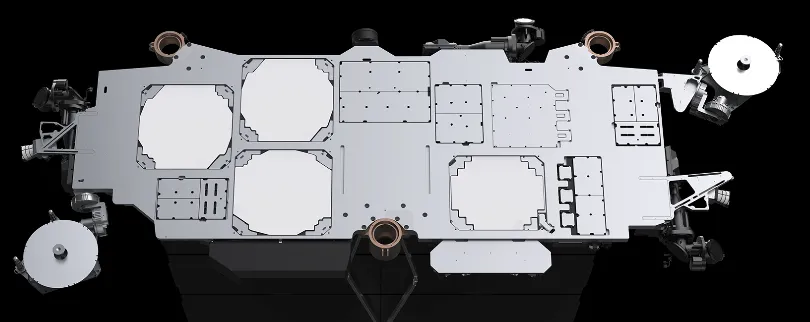
\includegraphics[width=0.9\linewidth]{./res/img/starlink_satellite_back.png}
  \caption{Fondo di un satellite Starlink \cite{mike_puchol_modeling_2022}}
  \label{fig:starlink-satellite}
\end{figure}

\subsubsection{Vincoli e limitazioni}
Ci sono alcune limitazioni, imposte dai regolatori, che riducono i livelli di servizio che il sistema Starlink può formire.

\paragraph{Riutilizzo di frequenze e fasci di co-frequenza a spot}
Qualsiasi satellite che emette energia tramite radiofrequenza verso la terra deve essere conforme con i limiti di potenza ricevuta a terra, misurati come Equivalent Power Flux Density (EPFD), stabiliti principalmente dall'\ac{ITU}.
La potenza dei fasci spot le cui impronte si sovrappongono e condividono la stessa frequenza è addittiva, quindi, per rispettare i limiti, la potenza di trasmissione di ciascun fascio deve essere ridotta.

In alcune aree, lo spettro \ac{Ka}-band disponibile per i gateway è ridotto alla metà, a causa dell'uso prioritario da parte di altri licenziatari. Ciò dimezza effettivamente la capaciità di troasmissione che ciascuno di questi gateway può fornire ai satelliti connessi \cite{mike_puchol_modeling_2022}

\subsection{Laser Inter Satellite Link}

Una recente aggiunta tecnologica per i satelliti Starlink, iniziando dalla versione 1.5 nel giugno 2021, è stata quella dei Laser Inter Satellite Links \ac{LISL}.
Ciascun satellite ha 3 terminali per la comunicazione, come mostrato in figura \ref{fig:starlink-ISL} \cite{mike_puchol_modeling_2022} \cite{chaudhry_laser_2021}.
Ci sono due tipi di \ac{LISL}:
\begin{itemize}
  \item \ac{LISL} intra-orbitali: per i collegamenti tra satelliti sullo stesso piano orbitale. Sono link permanenti dato che i satelliti si muovono tutti alla stessa velocità.
  \item \ac{LISL} inter-orbitali: per i collegamenti tra satelliti in piani orbitali diversi.
\end{itemize}

\begin{figure}[htbp]
  \centering
  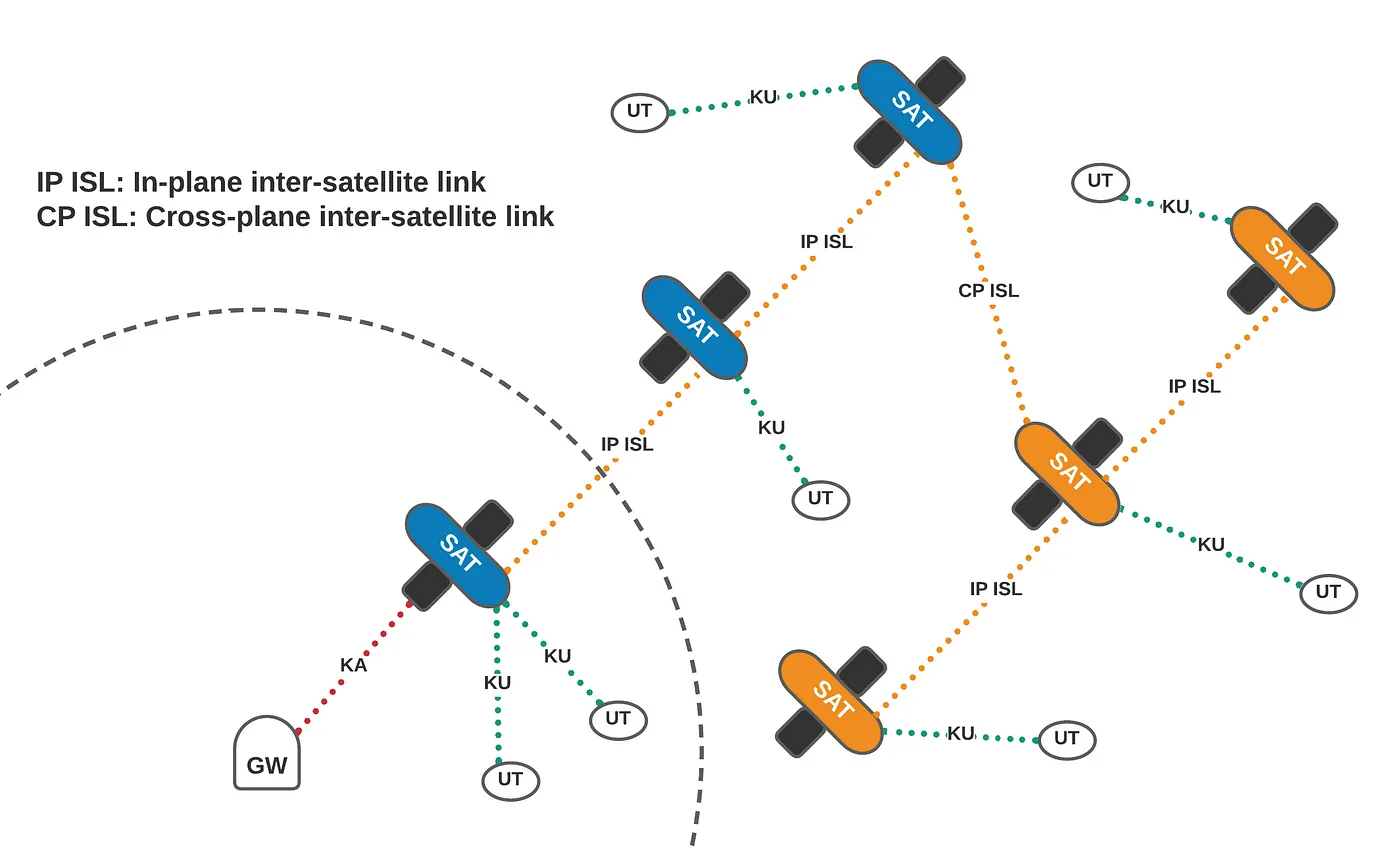
\includegraphics[width=0.9\linewidth]{./res/img/LISL_scheme.png}
  \caption{Schema dell'\ac{ISL} \cite{mike_puchol_modeling_2022}}
  \label{fig:starlink-ISL}
\end{figure}

In questo scenario, un satellite è connesso a un gateway.
Gli altri satelliti non hanno necessariamente connettività diretta al gateway, ma possono usare gli \ac{ISL} nello stesso piano e in piano incrociato per dirigere il traffico, e sono quindi in grado di servire terminali utente che non avrebbero altrimenti copertura.
Starlink ha inserito un'immagine di come sono fatti i terminali \ac{ISL}, che si può vedere in figura \ref{fig:starlink-terminal}.

\begin{figure}[htbp]
  \centering
  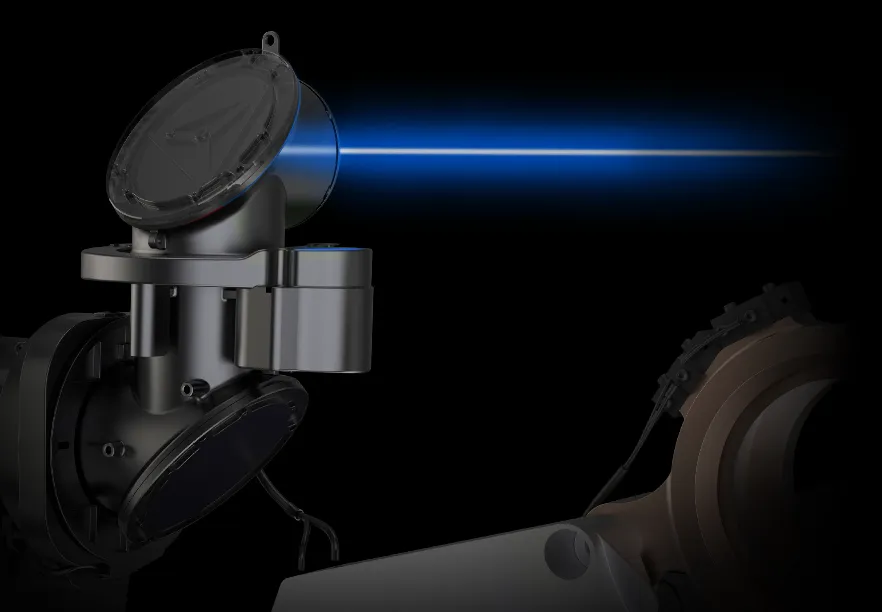
\includegraphics[width=0.9\linewidth]{./res/img/LISL_terminal.png}
  \caption{Terminale \ac{ISL} in un satellite \cite{mike_puchol_modeling_2022}}
  \label{fig:starlink-terminal}
\end{figure}

I \ac{LISL} facilitano la trasmissione di dati ad alta velocità tra satelliti in una costellazione, e sono cruciali per la rete Starlink per andare incontro alla crescente domanda di comunicazioni a bassa latenza ed alta capacità.
Adottare \ac{LISL} ha dei vantaggi rispetto ai classici collegamenti a radiofrequenza (\ac{RF}) \cite{chaudhry_laser_2021}.
\begin{itemize}
  \item Data rate più alti dato che si usano laser invece di link \ac{RF}.
  \item Dimensione e peso minore dato che l'utilizzo di laser consente di avere antenne più piccole, risultando in un peso e volume ridotto per i terminali di comunicazione, rendendoli più semplici da integrare nei satelliti.
  \item Migliore sicurezza dato che l'ampiezza ridotta del fascio laser riduce al minimo le interferenze e migliora la sicurezza rendendo più difficile l'intercettazione del segnale.
  \item Basso consumo energetico della tecnologia ottica.
\end{itemize}

Bisogna però ricordare che ci sono anche degli svantaggi.
Infatti, se un singolo piano orbitale con 20 satelliti condivide un gateway, ciascun satellite avrà un capacità bilanciata del $5\%$ di quella di un satellite indipendente.

Per ora la sfida principale rimane quella dei tempi di setup, dato che per stabilire un collegamento è richiesto da qualche secondo fino a decine di secondi \cite{chaudhry_laser_2021}.

\section{Segmento di terra}
I segmenti di terra includono diverse facilities che gestiscono la rete e forniscono connettività internet ai satelliti. Questi funzionano anche da Ground Station e sono localizzati strategicamente intorno al mondo per fornire copertura a zone remote e con poca connettività a internet.
La ground station è connessa all'\ac{ISP} tramite fibra \cite{branch_education_how_2022}.
Starlink ha anche preso accordi per installare stazioni di terra in prossimità di datacenter Google, di modo da fornire accesso veloce alle applicazioni e servizi più importanti \cite{jason_rainbow_starlink_2021}.

I satelliti passano il traffico verso un gateway utilizzando due antenne Phased Array in \ac{Ka}-band. Ogni gateway dispone in genere di nove antenne, in configurazione 3x3, 4x5 oppure 1x9 \cite{mike_puchol_modeling_2022}.

\begin{figure}[htbp]
  \centering
  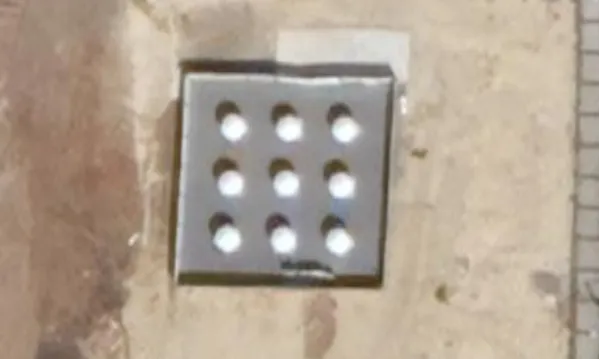
\includegraphics[width=0.9\linewidth]{./res/img/starlink_gateway.png}
  \caption{Configurazione 3x3 in Turchia \cite{mike_puchol_modeling_2022}}
  \label{fig:starlink-gateway}
\end{figure}

Solitamente otto antenne sono funzionanti, e una è tenuta come scorta.
Un gateway può quindi osservare completamente 4 satelliti \cite{mike_puchol_modeling_2022}.

Le due antenne paraboliche \ac{Ka} band combinate forniscono un throughput di circa 20 Gbps quando connesse a un gateway.
Ciascun antenna di un gateway ha un massimo di 4x500 MHz canali (2 GHz in totale) in uplink, e 5x250 MHz canali (1.25 GHz in totale) in downlink.

\begin{figure}[htbp]
  \centering
  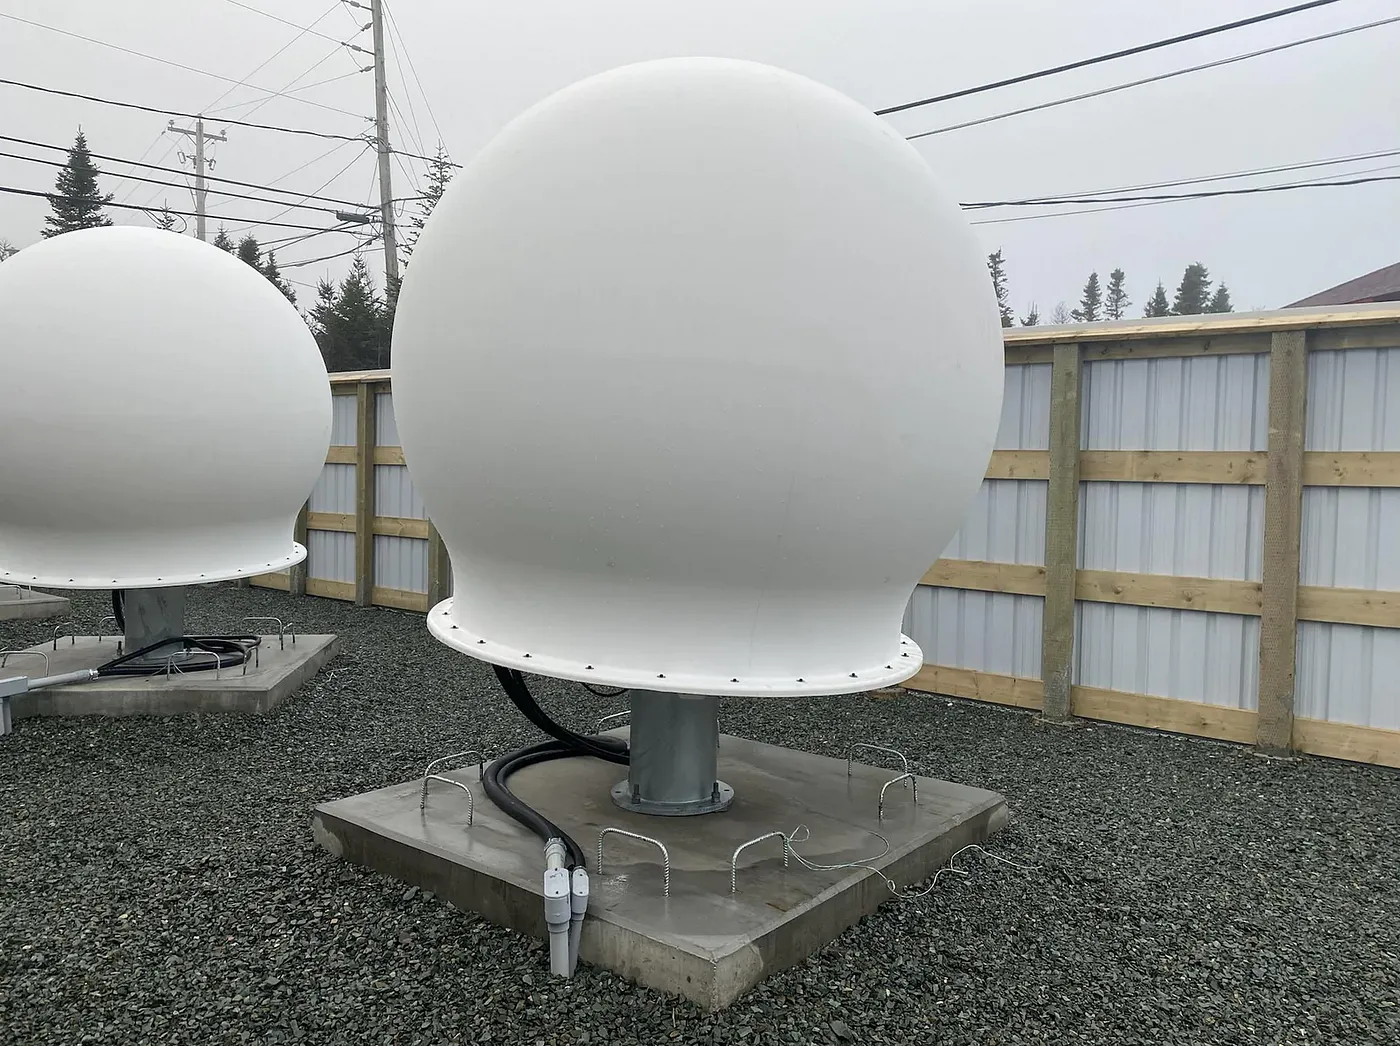
\includegraphics[width=0.9\linewidth]{./res/img/starlink_gateway_near.png}
  \caption{Una tipica antenna di gateway \cite{mike_puchol_modeling_2022}}
  \label{fig:starlink-gateway-near}
\end{figure}

\section{Segmento utente}
Il segmento utente comprende l'area in cui le persone utilizzano i servizi di ricezione Internet tramite il kit che viene fornito e che comprende l'antenna per la trasmissione, il cavo di alimentazione, il router (tranne nella versione mini dell'antenna dove il router è integrato all'antenna) e il cavo di rete per connettere l'antenna al router se quest'ultimo è incluso \cite{branch_education_how_2022}.

\begin{figure}[htbp]
  \centering
  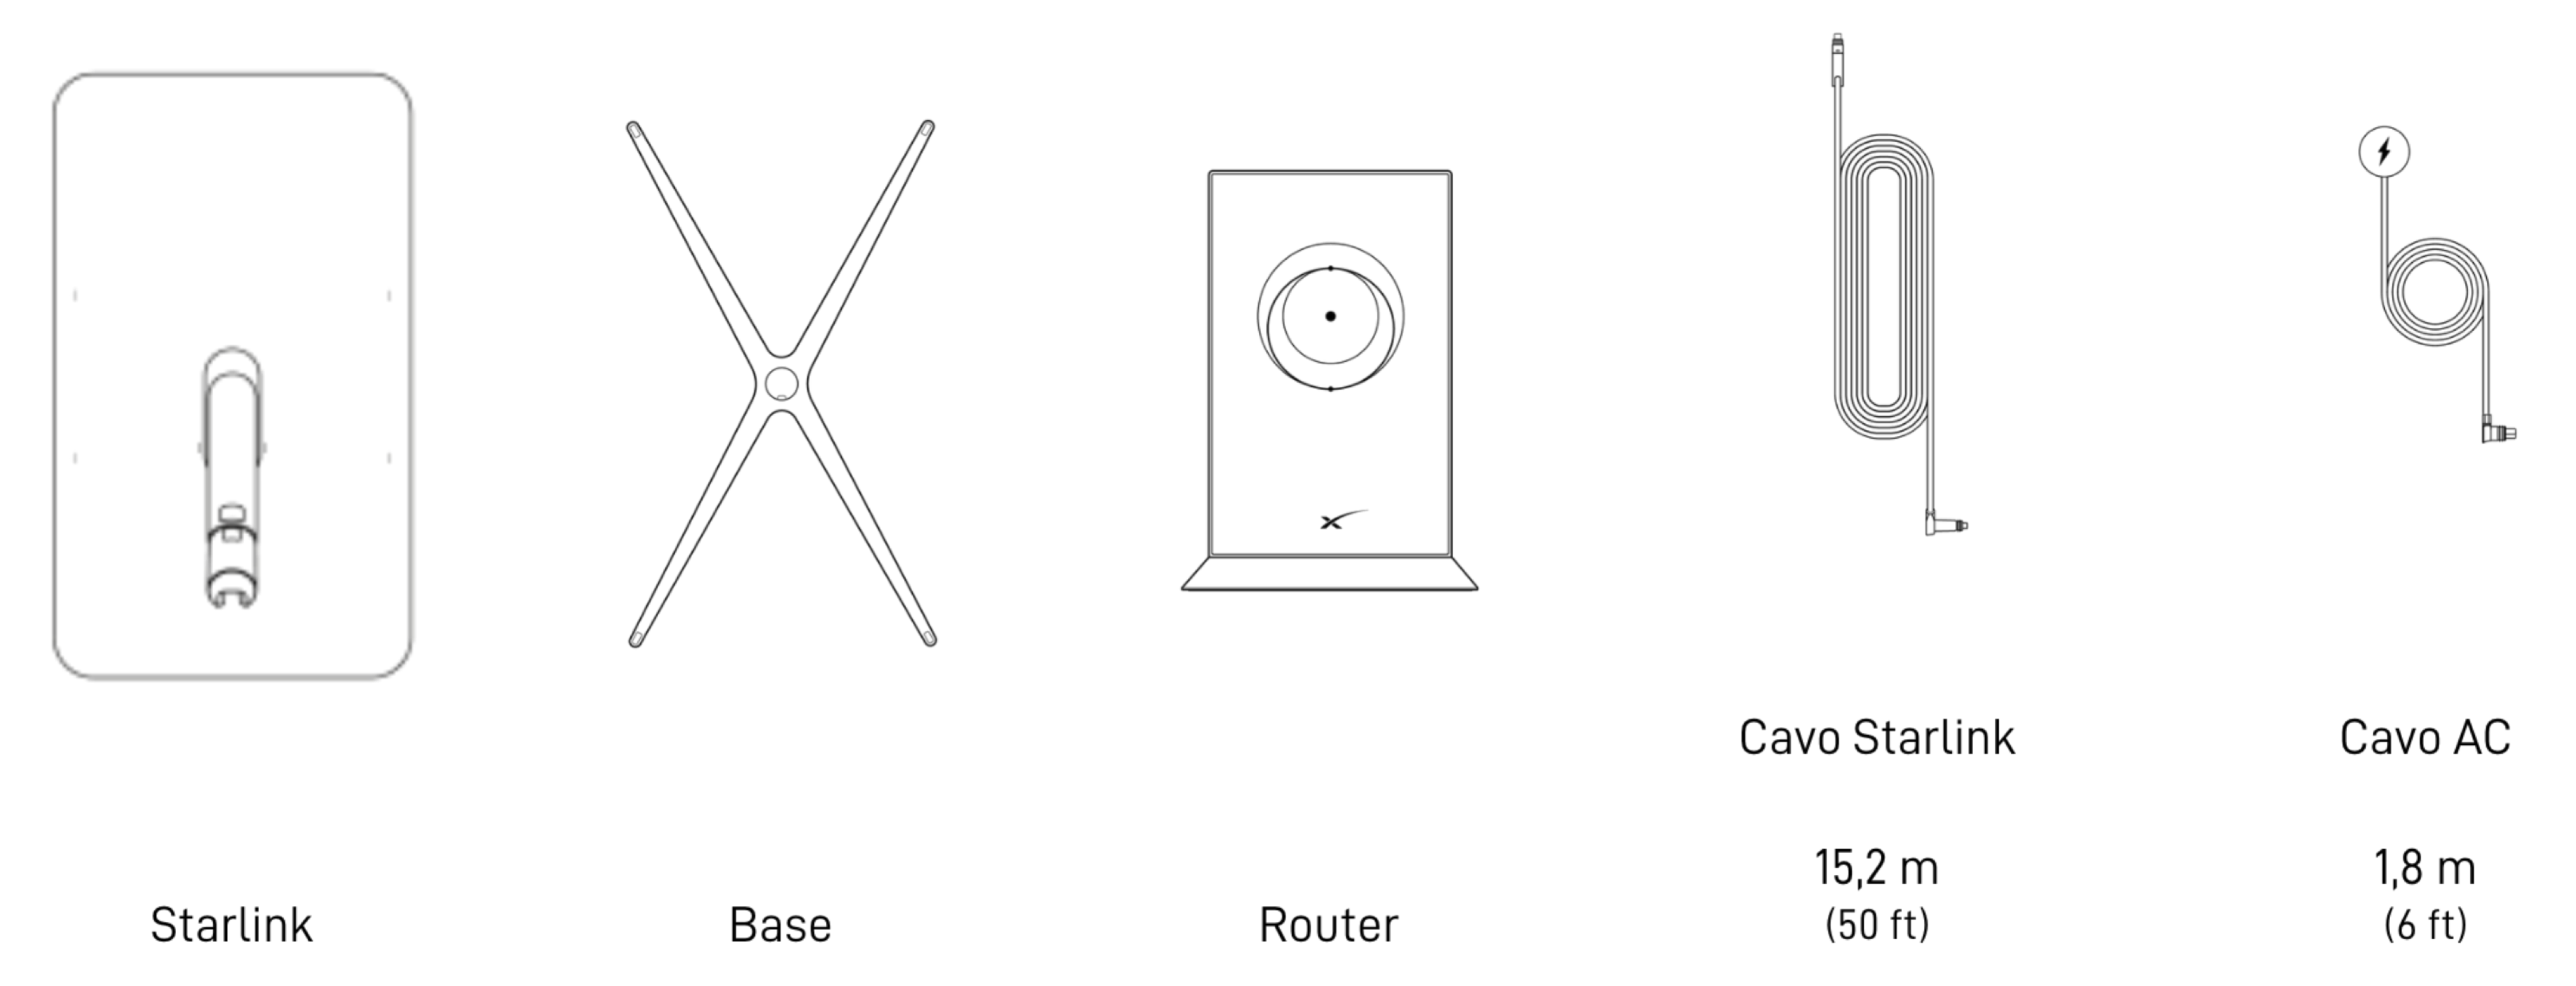
\includegraphics[width=0.8\linewidth]{./res/img/starlink_kit_standard.png}
  \caption{Contenuto della confezione del kit "standard actuated" \cite{starlink_specifiche_nodate}}
  \label{fig:starlink-kit-standard}
\end{figure}

L'antenna del kit "standard actuated" è un'antenna elettronica phased array, con orientamento motorizzato auto-orientante.
L'antenna ha una classificazione ambientale IP54 (Ingress Protection 54) che indica quanto bene un oggetto è protetto rispettivamente dalla polvere e dall'acqua.
Il livello 5 indica la protezione dalla polvere, il cui ingresso non è interamente impedito, ma la quantità che entra non è sufficiente per interferire con l'operazione sicura dell'antenna.
Invece il livello 4 per la protezione dall'acqua indica che schizzi d'acqua da qualsiasi direzione non hanno effetti dannosi sul funzionamento dell'antenna.
I gradi di protezione sono standardizzati dall'International Electrotechnical Commission.

L'antenna consuma in media dai 50 ai 75 W per il suo funzionamento, e anche grazie a questo riesce a sciogliere fino a 40 mm/ora di neve, che è molto utile per le condizioni avverse in cui spesso il servizio Starlink viene utilizzato.

Il router Wi-Fi invece supporta la generazione Wi-Fi 5, che supporta fino a 6.9 Gbps (massimo teorico) a 5 GHz.